\documentclass{ifacconf}

\usepackage{graphicx, color}
\usepackage{natbib}
\usepackage{amsmath,amssymb,amsfonts}
\usepackage{bbm}
\usepackage{amsfonts}
\usepackage{booktabs}
\usepackage{dsfont}
\usepackage{siunitx}
\usepackage{balance}
\usepackage{soul}
\usepackage{mathtools}
\usepackage{float}
\usepackage{tikz}
\usepackage{algorithm}
\usepackage{algpseudocode}
\algrenewcommand\algorithmicindent{1.0em}
% \usepackage{url}
\usepackage{xurl} % 依然用它来完美处理下划线换行
\usepackage[bookmarks=false, implicit=false, hidelinks]{hyperref} % 关闭书签和底层干涉，只保留点击跳转

% 告诉 LaTeX 允许在下划线 _ 和连字符 - 处将长 URL 断开
\makeatletter
\g@addto@macro{\UrlBreaks}{\do\_\do\-}
\makeatother

\newcommand{\cC} { {\mathcal C}}
\newcommand{\cM} { {\mathcal M}}
\newcommand{\cD} { {\mathcal D}}
\newcommand{\cK} { {\mathcal K}}
\newcommand{\cL} { {\mathcal L}}
\newcommand{\cS} { {\mathcal S}}

\newcommand{\bR} { {\mathbb R}}


\newcommand{\1}{\mbox{1}\hspace{-0.25em}\mbox{l}}

\def\red{\hfill $\lhd$}

\newcommand{\yk}[1]{{\color{blue}#1}}

\usetikzlibrary{arrows,automata,shapes,backgrounds,calc,positioning,patterns,decorations.pathmorphing,decorations.markings,mindmap,trees}
\tikzstyle{block} = [draw, rectangle, minimum height=2em, minimum
width=4em] \tikzstyle{sum} = [draw, fill=blue!20, circle, node
distance=1cm] \tikzstyle{input} = [coordinate] \tikzstyle{output} =
[coordinate] \tikzstyle{pinstyle} = [pin edge={to-,thin,black}]
\usepackage[american,cute inductors,smartlabels]{circuitikz}
\usetikzlibrary{calc}
\ctikzset{bipoles/thickness=1} \ctikzset{bipoles/length=0.8cm}
\ctikzset{bipoles/diode/height=.375}
\ctikzset{bipoles/diode/width=.3}
\ctikzset{tripoles/thyristor/height=.8}
\ctikzset{tripoles/thyristor/width=1}
\ctikzset{bipoles/vsourceam/height/.initial=.7}
\ctikzset{bipoles/vsourceam/width/.initial=.7} \tikzstyle{every
node}=[font=\small] \tikzstyle{every path}=[line width=0.8pt,line
cap=round,line join=round]



\begin{document}
\begin{frontmatter}

\title{Distributionally Robust Multi-Agent Reinforcement Learning for Intelligent Traffic Control}

\thanks[footnoteinfo]{This work was supported by the Holland High Tech (TKI HTSM) strategic program PPS-I Flex HighTech under the project number 24PPS173-CABS.}

\author[CN]{Shuwei Pei}
\author[CN]{Joran Borger}
\author[TK]{Arda Kosay}
\author[TK]{Muhammed O. Sayin}
\author[CN]{Saeed Ahmed}



\address[CN]{Engineering and Technology institute Groningen, Faculty of Science and Engineering, University of Groningen, 9747 AG Groningen, the Netherlands (e-mails: s.pei@rug.nl, j.borger.3@student.rug.nl, s.ahmed@rug.nl)}

\address[TK]{Department of Electrical, Electronics Engineering, Bilkent University, TR-06800 Ankara, Turkey (e-mail: arda.kosay@bilkent.edu.tr, sayin@ee.bilkent.edu.tr)}

\begin{abstract}
Learning-based traffic signal control optimized for average performance often degrades under atypical conditions. To address this, we propose a distributionally robust multi-agent reinforcement learning (DR-MARL) framework, evaluated on a $3\times 3$ Athens grid calibrated with pNEUMA trajectory data~\citep{BarmpounakisGeroliminis2020}. Our approach first trains a baseline MARL controller using proximal policy optimization. To capture demand uncertainty, we define eight heterogeneous origin-destination scenarios and train a contextual-bandit worst-case estimator to dynamically identify adversarial demand mixtures. Fine-tuning the baseline agents under these worst-case conditions yields our DR-MARL controller. Across all scenarios and an unseen Sioux Falls validation network, DR-MARL consistently improves upon the baseline, achieving up to 51\% shorter queues and 38\% higher speeds on the worst-performing scenarios.
\end{abstract}

\begin{keyword}
Reinforcement Learning; Distributionally Robust Optimization; Traffic Signal Control; Intelligent Transportation Systems.
\end{keyword}

\end{frontmatter}

\section{Introduction}

Urban intersections are major bottlenecks in road networks, disproportionately contributing to delay, economic loss~\citep{faheem2024impact}, and emissions~\citep{cohen2005global}. As urbanization increases pressure on transport systems~\citep{dijkstra2021applying}, designing signal control strategies that remain effective under uncertain traffic conditions becomes a central challenge.

Most existing systems rely on \emph{fixed-time}, \emph{actuated}, or rule-based \emph{adaptive} control. Classical schemes like SCOOT and SCATS provide efficient progression under nominal conditions~\citep{Hunt1982SCOOT,Luk1984SCATSCOOT}, but performance degrades during atypical flows. Actuated and adaptive schemes improve responsiveness yet remain largely myopic, struggling in dense networks with complex spillback and safety constraints~\citep{stevanovic2010atcs}.

Reinforcement learning (RL) offers a data-driven alternative, adapting signal timing via traffic interaction~\citep{sutton1998reinforcement}. Multi-agent RL (MARL) handles networks by assigning an agent to each intersection, coordinating via local observations to achieve promising results~\citep{zhang2023learning,huang2023reinforcement}. However, these methods are typically trained on nominal demand patterns and optimized for expected return, focusing only on average performance.
\begin{figure}[t!]
    \centering
    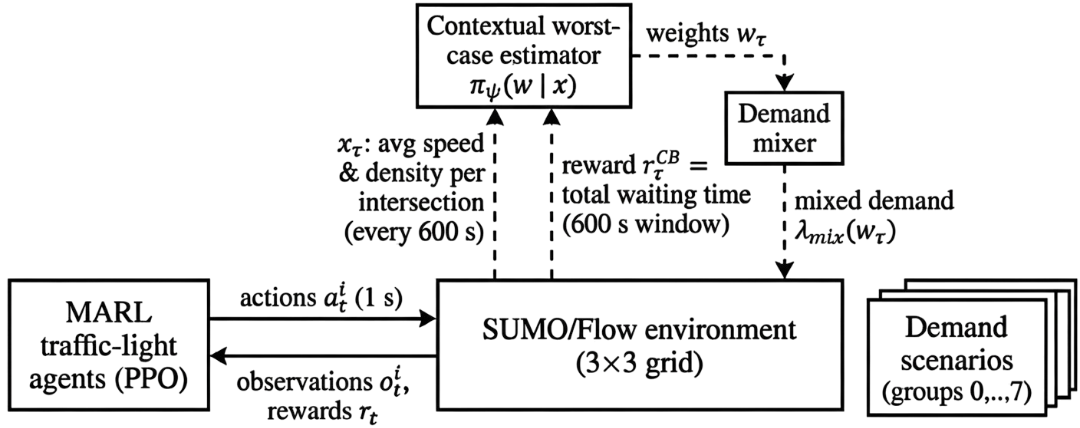
\includegraphics[width=1.0\linewidth]{overview_DR-MARL.png}
    \caption{Schematic of DR-MARL controller for intelligent intersection management.}
    \label{fig:overview}
\end{figure}
In practice, operators prioritize \emph{worst-case} behavior across diverse scenarios over average delay. Standard RL lacks tail guarantees, motivating robust formulations that upweight poorly performing scenarios~\citep{sagawa2020gdro}. To address this, we adopt a contextual-bandit worst-case estimator (CB-WCE)~\citep{liu2025distributionallyrobustmultiagentreinforcement} to adaptively reweight scenarios during training. This steers a standard MARL controller trained with proximal policy optimization (PPO) toward improved worst-case performance without changing the architecture. While robust RL methods are proven on abstract benchmarks~\citep{hashimoto2018fairness}, their transferability to network-level traffic control with strict safety constraints remains largely unexplored. We provide our source code and simulation environment to support reproducibility: \url{https://github.com/TravidP/DRMARL_CBWCE_Traffic_Controller}.


\textbf{Contribution:}
As shown in Fig.~\ref{fig:overview}, we employ a CB-WCE to reweight traffic scenarios during training, yielding a distributionally robust MARL (DR-MARL) controller without changing the underlying architecture. Concretely, our contributions are:
\begin{enumerate}
  \item We instantiate a MARL controller for a signalized \(3\times 3\) grid in a centralized training decentralized execution (CTDE) framework as our baseline MARL controller. It uses compact lane-based observations and discrete phase actions in a high-fidelity SUMO simulation environment.
  \item We propose a CB-WCE trained by OD-based demand patterns, enabling the generation of more variable and adversarial traffic scenarios for robust controller training.
  \item  We retrain the baseline MARL controller with a worst-case estimator, obtaining a DR-MARL policy, and compare its average and worst-case network performance (delay, queues, throughput) against the original MARL across various traffic scenarios.
 
\end{enumerate}



\textbf{Organization:}
Section~2 formulates the multi-agent traffic-signal control problem on the calibrated \(3\times 3\) grid and introduces the baseline MARL controller. Section~3 presents the scenario-based robustness objective, the CB-WCE, and the DR-MARL retraining procedure. Section~4 describes the experimental setup, including the network, traffic demand construction, and training protocol. Section~5 discusses numerical results, and Section~6 concludes the findings and outlines future work.




\section{Problem Setting and MARL Baseline}
\label{sec:problem}

\subsection{Network}
\label{subsec:network-signal}
We use a $3\times3$ signalized grid based on a subarea of central Athens from the pNEUMA dataset~\citep{BarmpounakisGeroliminis2020}. Real intersection coordinates are connected by straight links to preserve realistic scale and block lengths. Each bidirectional road segment has four lanes per direction. For the RL interface, we aggregate these into two movements per approach (N, S, E, W): a straight/right (SR) movement (lanes 0--1) and a left-turn (LT) movement (lanes 2--3, allowing U-turns).
\subsection{Traffic signal control as a multi-agent RL problem}
\label{subsec:marl-setting}

% We model network-wide traffic signal control on a $3\times3$ urban grid as a MARL problem. The grid geometry (link lengths, intersection spacing) is calibrated from a contiguous $3\times3$ subarea of central Athens covered by the pNEUMA trajectory dataset~\citep{BarmpounakisGeroliminis2020}, yielding realistic block lengths and intersection density. Traffic dynamics are simulated in \textsc{SUMO}~\citep{Krajzewicz2012SUMO} and interfaced via \textsc{FLOW}~\citep{Wu2021Flow} as a Markov decision process (MDP) for RL training. Details of the simulator stack and network construction are given in Section~\ref{sec:setup}.

On a $3\times3$ urban grid, we model each signalized intersection as a single learning agent, with all agents treated as homogeneous and sharing a common policy that is updated together.
Let $\mathcal{I}$ index the junctions, and let 
$t \in \{0,\dots,H-1\}$ denote discrete decision steps within an episode of length $H$. 
Denote by $z_t \in \mathcal{Z}$ the global traffic state at time $t$ and by 
$\mathbf{a}_t \coloneqq (a_t^i)_{i \in \mathcal{I}}$, the joint signal action over all intersections. 
The traffic state then evolves according to the Markovian dynamics:
$
z_{t+1} \sim 
P_{\mathrm{env}}\bigl(\,\cdot \mid z_t, \mathbf{a}_t \bigr),
$
where the transition kernel $P_{\mathrm{env}}$ is induced by \textsc{SUMO}'s microscopic vehicle dynamics and the signal programs.


\textbf{Observation.} For each intersection $i \in \mathcal{I}$, the observation $o_t^i = f_i(s_t)$ summarizes traffic and signal conditions in a local neighborhood. On the traffic side, we track eight aggregated lane movements (straight/right (SR), and left-turn (LT) for North/South/East/West) and, for each movement, record eight features: a movement identifier (SR vs.\ LT), distances and speeds of the closest and second-closest vehicle to the intersection, lane density, mean speed, and a queue fraction (fraction of vehicles with $v < 0.1$\,\si{m/s}, normalized to a 10-vehicle queue). This yields $8\times 8 = 64$ traffic features. In addition, the agent obtains basic signal-state information for the controlled intersection and its four orthogonal neighbors: time since last phase change, current phase index, and a flag indicating whether the signal is in a yellow/all-red (clearance) interval, giving $5\times 3 = 15$ signal features. Together, these form a compact observation vector
\(
o_t^i \in \mathbb{R}^{79},
\)
designed to capture local pressure and limited neighborhood context.

\textbf{Action and safety.}
At each decision step, agent $i$ selects a discrete action $a_t^i \in \{0,\dots,7\}$, choosing one of eight non-conflicting signal phases at that junction. The phase set covers straight/right movements for the north--south and east--west pairs, protected left turns for these pairs, and four single-approach phases where all movements (SR+LT) on one approach receive green. Safety is enforced via a fixed \SI{5}{s} clearance interval (yellow plus all-red) applied whenever a phase changes, ensuring that vehicles clearing the intersection are never exposed to newly conflicting movements. When switching between phases, we allow ``green carryover'' for movements that are green in both the old and new phase, avoiding unnecessary clearance for non-conflicting streams and improving throughput.

\textbf{Reward.}
The agents are homogeneous and share the same local reward specification. 
At every step $t$, each agent $i$ receives a local reward $r_t^i$ defined over vehicles on its incoming edges. 
The reward combines two components: (i) a normalized mean-speed term promoting throughput, and (ii) a penalty on normalized queue length. 
Concretely, we use
$r_t^i
= \kappa_s \, s_i
- \kappa_q \, \bar q_i,$
where $s_i$ is the normalized mean speed on incoming edges, $\bar q_i$ is a normalized queue measure, and the weights $\kappa_s,\kappa_q$ are shared across all agents.
To train the homogeneous shared policy, we use a single team reward given by the sum of local rewards,
$r_t \;=\; \sum_{i\in\mathcal{I}} r_t^i,$
which provides a common learning signal for all agents.


% \subsection{Traffic demand}
% \label{subsec:baseline_demand}






\subsection{PPO-based MARL controller (baseline)}
\label{subsec:ppo-baseline}

For baseline training, we adopt a CTDE scheme with parameter sharing.
All homogeneous intersections share a stochastic policy $\pi_\theta : \mathcal{O} \to \Delta(\mathcal{A})$,
with each agent $i$ executing decentralized actions $a_t^i \sim \pi_\theta(\cdot \mid o_t^i)$ based on local observations.
During training, trajectories and rewards from all agents are aggregated to jointly update $\theta$.
This parameter-sharing CTDE design exploits intersection homogeneity, improving sample efficiency and reducing trainable parameters.



Let $\tau = (s_0,o_0^{1:|\mathcal{I}|},a_0^{1:|\mathcal{I}|},r_0,\dots,s_{H})$ denote a trajectory induced by $\pi_\theta$ and the environment dynamics, where $o_t^{1:|\mathcal{I}|} := (o_t^1,\dots,o_t^{|\mathcal{I}|})$ and similarly for $a_t^{1:|\mathcal{I}|}$. The baseline objective maximizes the expected discounted return over the training distribution of traffic scenarios:
\begin{equation}
J(\theta)
\;=\;
\mathbb{E}_{\tau \sim \pi_\theta}
\Bigg[
\sum_{t=0}^{H-1} \gamma^{t} \, r_t
\Bigg],
\label{eq:global-objective}
\end{equation}
with discount factor $\gamma\in(0,1]$. In this baseline, the demand pattern is fixed to the static distribution; the controller is not yet biased toward worst-case conditions.

We optimize~\eqref{eq:global-objective} using PPO~\citep{schulman2017proximal}, a clipped policy-gradient method that is widely used in continuous-control and multi-agent settings. 
Given a mini-batch 
$B$ sampled from the replay buffer $\mathcal{D}_\theta$, 
we define the policy-gradient objective
\begin{equation}
\begin{aligned}
    J(\theta; B)
    &:= 
    \frac{1}{|B|\,|\mathcal{I}|}
    \sum_{(o_t^i, a_t^i, r_t, o_{t+1}^i)\in B}
    \sum_{i\in\mathcal{I}}
        r_t \,\log \pi_\theta(a_t^i \mid o_t^i).
\end{aligned}
\end{equation}
The policy parameters are then updated by ascending the stochastic gradient 
$\nabla_\theta J(\theta; B)$.
Coordination emerges from local observations and the use of a homogeneous, parameter-shared policy. In Section~\ref{sec:method}, we build on this baseline by introducing a CB-WCE that reweights demand scenarios during training, effectively biasing learning toward worst-case conditions, while keeping the underlying PPO objective~\eqref{eq:global-objective} and architecture unchanged.







% ---------------------- New section ---------------------------






\section{Distributionally Robust MARL via Worst-Case Estimation}
\label{sec:method}


\subsection{Scenario-based robustness objective}
\label{subsec:robust-objective}

In our setting, it yields a finite set of $K$ representative traffic-demand scenarios,
corresponding to synthetic data with a distinct spatial flow pattern (e.g., different directional imbalances or overall loading). For a fixed MARL policy $\pi_\theta$ and a given scenario $k \in \mathcal{K}$, we define
\[
J_k(\theta)
\;=\;
\mathbb{E}\big[ R(\tau) \,\big|\, \text{scenario } k,\; \pi_\theta \big],
\]
as the expected return when the network is operated under that scenario, where $\tau$ denotes a time window $T_{\mathrm{win}}$ rollout trajectory and $R(\tau)$ its cumulative reward (a negative delay-based proxy) during the window $T_{\mathrm{win}}$. From these per-scenario returns we derive two evaluation metrics:
\begin{equation}
J_{\mathrm{avg}}(\theta)
\;=\;
\frac{1}{K} \sum_{k \in \mathcal{K}} J_k(\theta),
\qquad
J_{\mathrm{worst}}(\theta)
\;=\;
\min_{k \in \mathcal{K}} J_k(\theta).
\label{eq:j-avg-worst}
\end{equation}
Here $J_{\mathrm{avg}}$ captures typical performance across the eight scenarios, while $J_{\mathrm{worst}}$ captures performance under the most challenging one.

In our experiments, the baseline MARL controller is trained only under the synthetic, spatially balanced demand described in Section~\ref{sec:problem}. The baseline may perform well near its training distribution but degrade on some of the data-driven scenarios, leading to a low $J_{\mathrm{worst}}$. Our goal is to improve $J_{\mathrm{worst}}(\theta)$ and, ideally, to also improve $J_{\mathrm{avg}}(\theta)$ by retraining the MARL policy under traffic-demand patterns that are deliberately chosen to be difficult.
To this end, we introduce a CB-WCE that adaptively reweights the traffic-demand scenarios so that training is increasingly focused on those that induce high delay. 



\subsection{Contextual-bandit worst-case estimator}
\label{subsec:cb-estimator} The \emph{worst-case estimator} operates on a slower timescale than the traffic-signal MARL controller. Conceptually, this agent plays an adversarial role: for a fixed signal-control policy $\pi_\theta$, it tries to select traffic-demand patterns that \emph{maximize} network-wide congestion, so that subsequent updates of $\pi_\theta$ are biased toward difficult conditions. The estimator acts once every window $T_{\mathrm{win}}$, while the traffic-light agents act every simulation second.


\textbf{Observation.}
At the end of window $T_{\mathrm{win}}$, we summarize the recent network state by an 18-dimensional feature vector
\(
s_\tau \in \mathbb{R}^{18},
\)
constructed from the average speed and average density at each of the nine intersections (two scalars per intersection). It provides coarse information about where congestion currently occurs in the grid.

\textbf{Action.}
Given the window-level observation $x_\tau$, the estimator outputs a non-negative weight vector
\[
w_\tau \in \mathbb{R}_{\ge 0}^K, \qquad \sum_{k=1}^K w_{\tau,k} = 1.
\]
with one component $w_{\tau,k}$ for each of traffic-demand scenarios. These weights define a \emph{mixed} demand pattern for the next window $T_{\mathrm{win}}$ by combining the base inflow vectors $\{\lambda^{(k)}\}_{k=1}^K$ extracted from the inflow data:
\[
\lambda_{\mathrm{mix}}(w_\tau) \;=\; \sum_{k=1}^K w_{\tau,k} \,\lambda^{(k)}.
\]
The resulting mixed inflows are then applied in the next window.

\textbf{Reward.}
% During window $\tau{+}1$, the MARL traffic-light policy $\pi_\theta$ is applied at every second while demand is generated according to $\lambda_{\mathrm{mix}}(w_\tau)$. 
Over this window $T_{\mathrm{win}}$, we accumulate the total waiting time of all vehicles in the network,
\(
r_\tau^{\text{CB}} = \sum_{v} t_{\text{wait}, v}
\)
where $t_{\text{wait}, v}$ is the time vehicle $v$ spends queued in this time window $T_{\mathrm{win}}$. The CB-WCE seeks to \emph{maximize} this cumulative waiting time.

The worst-case estimator’s policy $\pi_\psi(w \mid s)$ is parameterized by a neural network and trained with a policy-gradient method. 
Here, $\pi_\psi(w_\tau \mid s_\tau)$ denotes a probability distribution over a weight vector for different traffic-demand scenarios, conditioned on the current local observation. As shown in Algorithm~\ref{alg:worst}, training is carried out with $\theta$ frozen at $\theta_0$, using tuples $(s_\tau,w_\tau,r_\tau^{\mathrm{CB}})$ collected over successive windows. Given a mini-batch 
$B$ 
sampled from the replay buffer $\mathcal{D}_w$, we define the contextual-bandit objective
\begin{equation}
    J_{\mathrm{CB}}(\psi; B)
    :=
    \frac{1}{|B|}
    \sum_{(s_\tau, w_\tau, r_\tau^{\mathrm{CB}}, s_{\tau+1}) \in B}
    r_\tau^{\mathrm{CB}} \,\log \pi_\psi(w_\tau \mid s_\tau),
\end{equation}
and update the estimator parameters via ascending the stochastic gradient 
$\nabla_\psi J_{\mathrm{CB}}(\psi; B)$., yielding a policy $\pi_{\psi^\ast}$ that focuses on adverse traffic-demand mixtures. 


% If we implement algorithm for worst case estimator it should come here
% \begin{algorithm}[H]
% \caption{\tiny Contextual Worst-Case Estimator}
% \begin{algorithmic}[1]

% \State \textbf{Input:} Traffic-demand scenarios $\mathcal{G}=\{g_j\}_{j=1}^J$;
% learning rate $l_w$; exploration rate $\epsilon_w$;
% group window length $T_{\mathrm{group}}$;
% pre-trained traffic-light controller $\pi_\theta$;
% replay buffer $\mathcal{D}_w$.

% \State \textbf{Output:} Learned estimator $Q_w(\cdot;\psi^\ast)$.

% \State Initialize estimator parameters $\psi$ and replay buffer $\mathcal{D}_w \gets \emptyset$.

% \For{episode $=1,\dots,K$}
%     \State Reset SUMO/Flow network; 
%     \State Warm up under random mixture $g' = \sum_j \alpha_j g_j$.
%     \State Observe initial network state $s_0$.

%     \For{window index $\tau = 0,\dots,$ until episode horizon}
        
%         \State With probability $\epsilon_w$: sample $g' \sim \mathrm{Uniform}(\mathcal{G})$.
%         \State Otherwise: $g' \gets \arg\max_{g\in\Delta(\mathcal{G})} Q_w(s_\tau, g;\psi)$.
        
%         \State Construct mixed demand $\lambda_{\mathrm{mix}}(g')$.

%         \State Initialize window reward $R_\tau \gets 0$.

%         \For{$t=1,\dots,T_{\mathrm{group}}$}
%             \For{each intersection $i=1,\dots,N$}
%                 \State Observe local state $o_t^i$.
%                 \State Select phase $a_t^i = \pi_\theta(o_t^i)$.
%             \EndFor

%             \State Apply $(a_t^1,\dots,a_t^N)$ under demand $g'$.
%             \State Compute $t_{\mathrm{wait}}$ at step $t$.
%             \State $R_\tau \gets R_\tau + t_{\mathrm{wait}}$.
%         \EndFor

%         \State Observe next state $s_{\tau+1}$.
%         \State Store $(s_\tau, g', R_\tau, s_{\tau+1})$ into $\mathcal{D}_w$.

%         \State Sample mini-batch $B \sim \mathcal{D}_w$.
%         \State Update $\psi \gets \psi + l_w \nabla_\psi J_w(\psi; B)$.

%         \State Decay $\epsilon_w$.
%     \EndFor
% \EndFor

% \end{algorithmic}
% \end{algorithm}

\begin{algorithm}[t!]
\caption{Contextual-bandit worst-case estimator}
\label{alg:worst}
\begin{algorithmic}[1]

\State \textbf{Input:} OD--based group distributions $\{\lambda^{(k)}\}_{k=1}^8$;
traffic-light controller policy $\pi_\theta$;
window length $T_{\mathrm{win}}$;
learning rate $l_\psi$;
episode horizon $H_{\mathrm{W}}$;
replay buffer $\mathcal{D}_w$.

\State \textbf{Output:} Worst-case estimator policy $\pi_{\psi^\ast}(w \mid s)$.

\State Initialize policy parameters $\psi$ and buffer $\mathcal{D}_w \gets \emptyset$.

\For{episode $=1,\dots,K$}
    \State Reset SUMO/Flow network.
    \State Warm up under a random mixture of $\{\lambda^{(k)}\}$.
    \State Compute initial observation $s_0$ 

    \For{group window index $\tau = 0,\dots,$ until $\mathcal{D}_w$}
        \State Sample weights $w_\tau \sim \pi_\psi(\cdot \mid s_\tau)$.
        \State Construct group $\lambda_{\mathrm{mix}}(w_\tau) = \sum_{k=1}^8 w_{\tau,k}\lambda^{(k)}$.
        \State Apply $\lambda_{\mathrm{mix}}(w_\tau)$ for the next $T_{\mathrm{win}}$ seconds.

        \State Initialize window reward $r_\tau^{\mathrm{CB}} \gets 0$.
        \For{$t = 1,\dots,T_{\mathrm{win}}$}
            \For{each intersection $i \in \mathcal{I}$}
                \State Observe $o_t^i$ and select $a_t^i \sim \pi_{\theta_0}(\cdot \mid o_t^i)$.
            \EndFor
             \State Apply $(a_t^i)_{i\in\mathcal{I}}$ under demand $\lambda_{\mathrm{mix}}(w_\tau)$.
            \State Compute waiting time $t_{\mathrm{wait}}$ of each vehicle at $t$.
            
            \State Accumulate $r_\tau^{\mathrm{CB}} \gets r_\tau^{\mathrm{CB}} +t_{\mathrm{wait}}$.
        \EndFor

        \State Compute next estimator observation $s_{\tau+1}$.
        \State Store $(s_\tau, w_\tau, r_\tau^{\mathrm{CB}}, s_{\tau+1})$ in $\mathcal{D}_w$.

    \EndFor
    \State Sample mini-batch $B \sim \mathcal{D}_w$.
    \State Update $\psi \gets \psi + l_\psi \nabla_\psi J_{\mathrm{CB}}(\psi; B)$.
\EndFor

\end{algorithmic}
\end{algorithm}

\subsection{DR-MARL training with a frozen worst-case estimator}
\label{subsec:drmarl}

We now describe how the CB-WCE is used to obtain a DR-MARL controller. As shown in Algorithm~\ref{alg:DRMARL}, after training the baseline MARL controller $\pi_{\theta_0}$ on the static, spatially balanced demand and training the contextual-bandit estimator $\pi_{\psi^\ast}(w \mid x)$ against this frozen baseline (Section~\ref{subsec:cb-estimator}), we initialize the DR-MARL controller with $\theta = \theta_0$ and perform an additional PPO fine-tuning phase in which only $\theta$ is updated. The CB-WCE $\pi_{\psi^\ast}$ is kept fixed and serves as a scheduler that selects mixed demand patterns during this retraining.

During DR-MARL fine-tuning, each training episode is partitioned into windows of length $T_{\mathrm{win}}$. At the beginning of window $T_{\mathrm{win}}$, we compute the observation $x_\tau$ (average speed and density at each intersection over the preceding window, or over an initial warm-up period for $\tau = 0$) and query the frozen estimator to obtain demand weights
$w_\tau \sim \pi_{\psi^\ast}(\cdot \mid x_\tau),$
which define the mixed demand pattern $\lambda_{\mathrm{mix}}(w_\tau)$ for the upcoming $T_{\mathrm{win}}$ seconds. Within this window, the MARL controller applies actions $a_t^i \sim \pi_\theta(\cdot \mid o_t^i)$ at every intersection $i$ each simulation second, while vehicles are generated according to $\lambda_{\mathrm{mix}}(w_\tau)$ and rewards $r_t$ are collected exactly as in the baseline setup. After all windows of an episode have been simulated, the resulting trajectory contributes to a PPO update of $\theta$ following the same setting in Section~\ref{subsec:ppo-baseline}. The policy parameters are then updated by ascending the stochastic gradient 
$\nabla_\theta J(\theta; B)$. Episodes are repeatedly generated in this two-timescale fashion, so that the traffic-signal policy gradually adapts to the adversarially chosen mixture of demand scenarios.

\begin{algorithm}[t!]
\caption{DR-MARL with a worst-case estimator}
\label{alg:DRMARL}
\begin{algorithmic}[1]
\State \textbf{Input:} Worst estimator $\pi_{\psi^\ast}(w \mid x)$;
baseline MARL policy parameters $\theta_0$;
OD--based group distributions $\{\lambda^{(k)}\}_{k=1}^8$
window length $T_{\mathrm{win}}$;
episode horizon $H_{\mathrm{DR}}$;
PPO learning rate $l_\theta$.

\State \textbf{Output:} Distributionally robust MARL policy $\pi_{\theta^\ast}$.

\State Initialize policy parameters $\theta \gets \theta_0$ and replay buffer $\mathcal{D}_\theta$.

\For{episode $=1,\dots,K_{\mathrm{DR}}$}

    \State Reset SUMO/Flow network.
    \State Warm up using a random mixture of $\{\lambda^{(k)}\}$.
    \State Compute initial estimator observation $x_0$.


    \For{group window index $\tau = 0,\dots,$ until $H_{\mathrm{DR}}$}

        \State Sample actions $w_\tau \sim \pi_{\psi^\ast}(\cdot \mid x_\tau)$.
        \State Construct group $\lambda_{\mathrm{mix}}(w_\tau) = \sum_{k=1}^8 w_{\tau,k}\lambda^{(k)}$.
        \State Apply $\lambda_{\mathrm{mix}}(w_\tau)$ for the next $T_{\mathrm{win}}$ seconds.

        \For{$t = 1,\dots,T_{\mathrm{win}}$}
            \For{each intersection $i \in \mathcal{I}$}
                \State Observe $o_t^i$ and sample $a_t^i \sim \pi_\theta(\cdot \mid o_t^i)$.
            \EndFor
            \State Apply $(a_t^i)_{i\in\mathcal{I}}$ under demand $\lambda_{\mathrm{mix}}(w_\tau)$.
            \State Compute $r_t$ and next observations $\{o_{t+1}^i\}_{i\in\mathcal{I}}$.
            \State Store $\big(\{o_t^i\}_{i\in\mathcal{I}}, \{a_t^i\}_{i\in\mathcal{I}}, r_t, \{o_{t+1}^i\}_{i\in\mathcal{I}}\big)$ in $\mathcal{D}_\theta$.
        \EndFor

        \State Compute next estimator observation $x_{\tau+1}$.

    \EndFor
    \State Sample mini-batch $B \sim \mathcal{D}_\theta$.
    \State Update $\theta \gets \theta + l_\theta \nabla_\theta J(\theta; B)$.

\EndFor

\end{algorithmic}
\end{algorithm}





% ---------------------- New section ---------------------------








\section{Experimental Setup}
\label{sec:setup}


\subsection{Traffic demand}
\label{subsec:demand}
For initial training of the baseline policy, we use an even traffic distribution over the outer edges of  $3\times3$ grid. Each outer edge acts as an origin, with a fixed inflow of \SI{400}{veh/h}, resulting in a total demand of \SI{4800}{veh/h}. For every vehicle spawned at origin $o$, the destination $d$ is sampled uniformly from the remaining $11$ outer edges, so that
$\Pr\{d \mid o\} = \tfrac{1}{11}, \quad d \neq o.$
Routes between each origin–destination pair follow shortest paths in edge count (breaking ties uniformly at random). This yields a balanced training distribution where all directions and origin–destination (OD) pairs are represented. 

To train the worst-case estimator and DR-MARL controller, we create a diverse set of eight origin-destination (OD) demand patterns for the $3{\times}3$ grid's 12 outer edges. One pattern is data-driven, derived from the pNEUMA trajectory dataset~\citep{BarmpounakisGeroliminis2020} by aggregating trip counts and normalizing to a total demand of \SI{5000}{veh/h}. To probe robustness, we add seven synthetic patterns with the same total inflow but varied spatial structures (e.g., uniform, inbound/outbound, corridor, and cross-town flows). This set of eight scenarios ($\mathcal{K}$ = 8) is used by the worst-case estimator to generate adversarial demand mixtures during training.


\begin{figure*}[t!]
    \centering
    \begin{minipage}{0.48\textwidth}
        \centering
        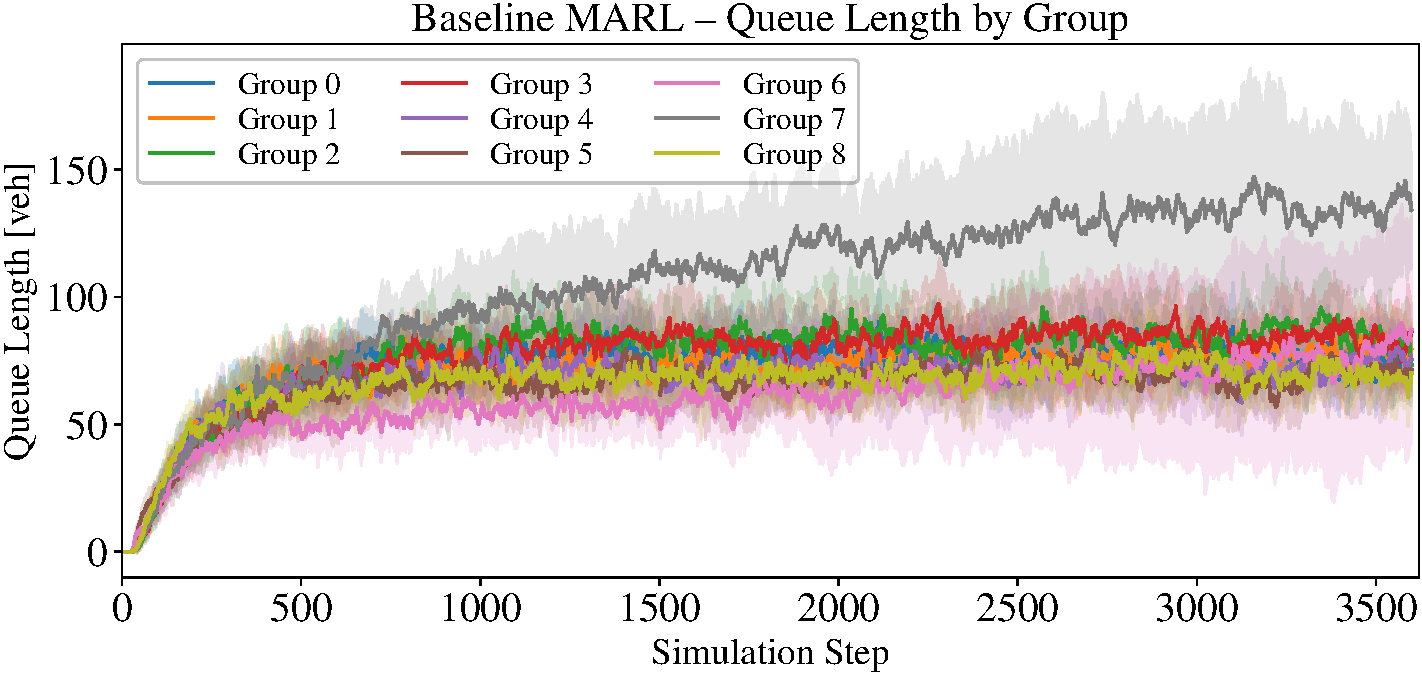
\includegraphics[width=1.0\linewidth]{baseline_queue_by_group.pdf}
        \caption{Queue length over time under MARL.}
        \label{fig:queue_baseline}
    \end{minipage}\hfill
    \begin{minipage}{0.48\textwidth}
        \centering
        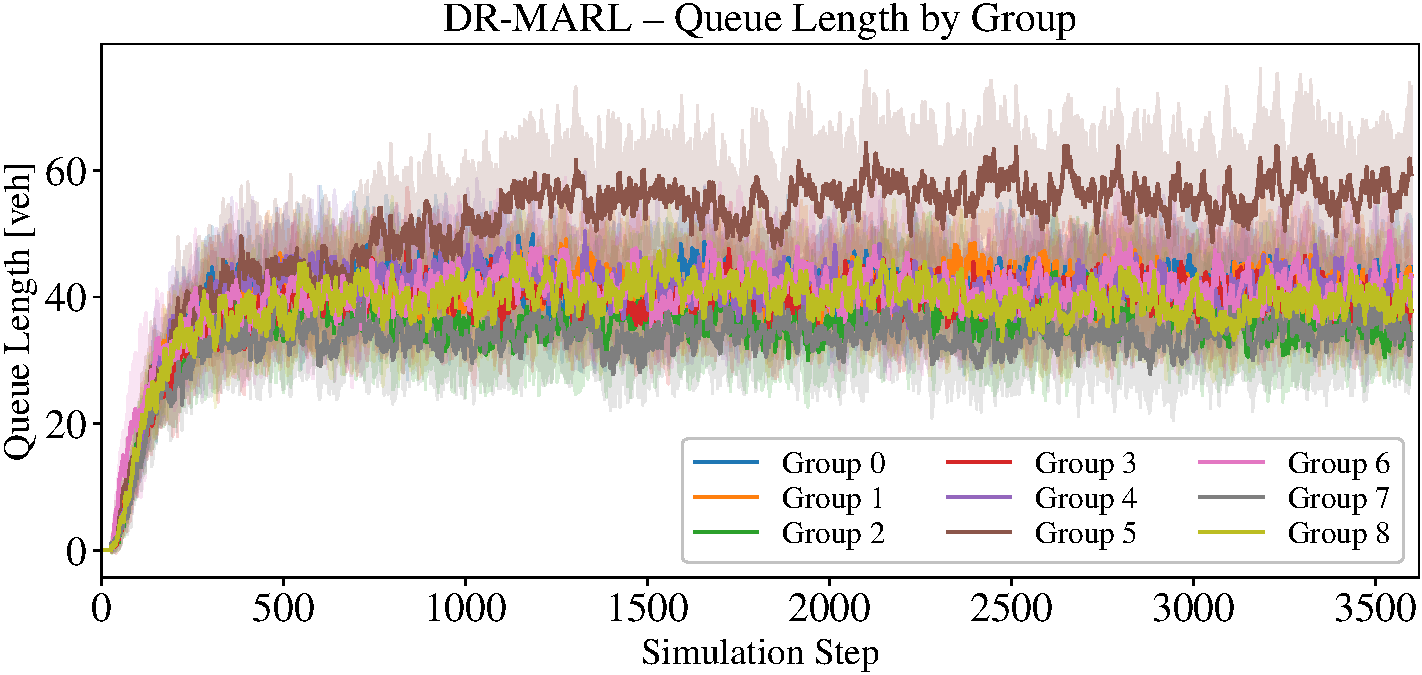
\includegraphics[width=1.0\linewidth]{drmarl_queue_by_group.pdf}
        \caption{Queue length over time under DR-MARL.}
        \label{fig:queue_robust}
    \end{minipage}
\end{figure*}
\begin{figure*}[t!]
    \centering
    \begin{minipage}{0.48\textwidth}
        \centering
        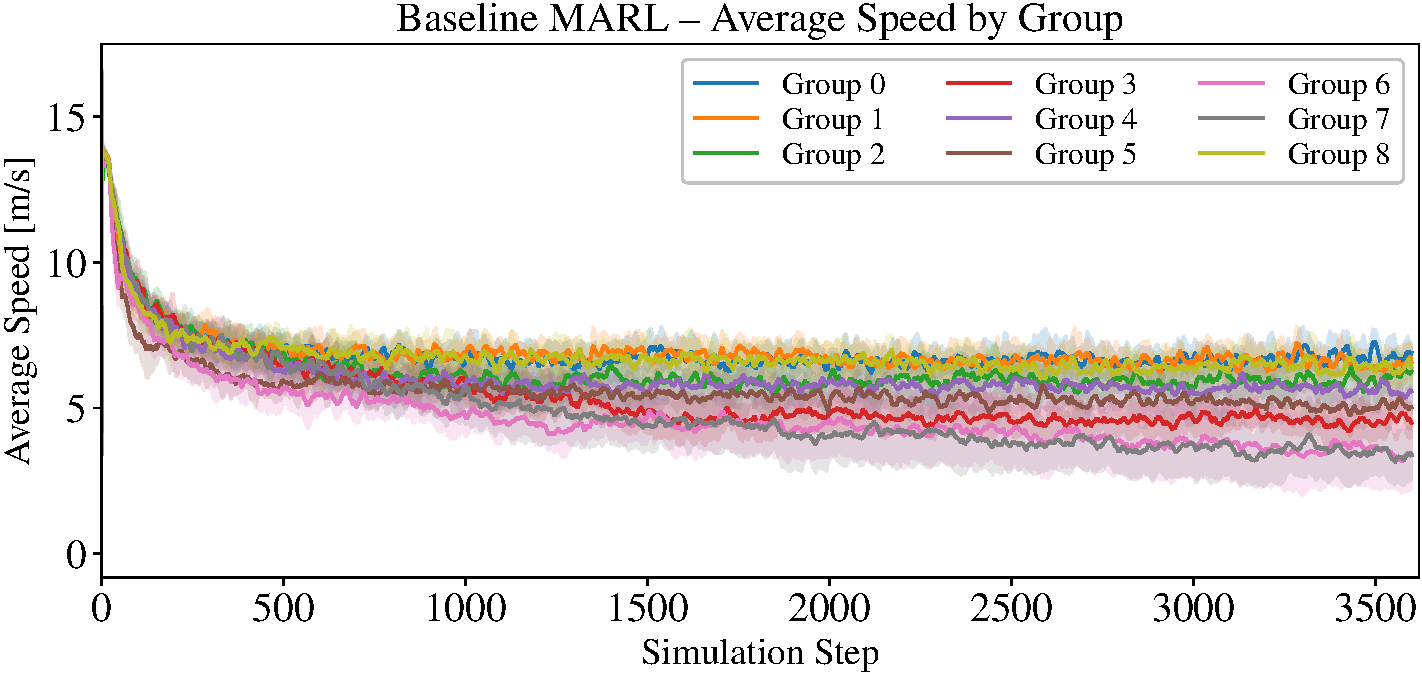
\includegraphics[width=1.0\linewidth]{baseline_speed_by_group.pdf}
        \caption{Average speed over time under MARL.}
        \label{fig:speed_baseline}
    \end{minipage}\hfill
    \begin{minipage}{0.48\textwidth}
        \centering
        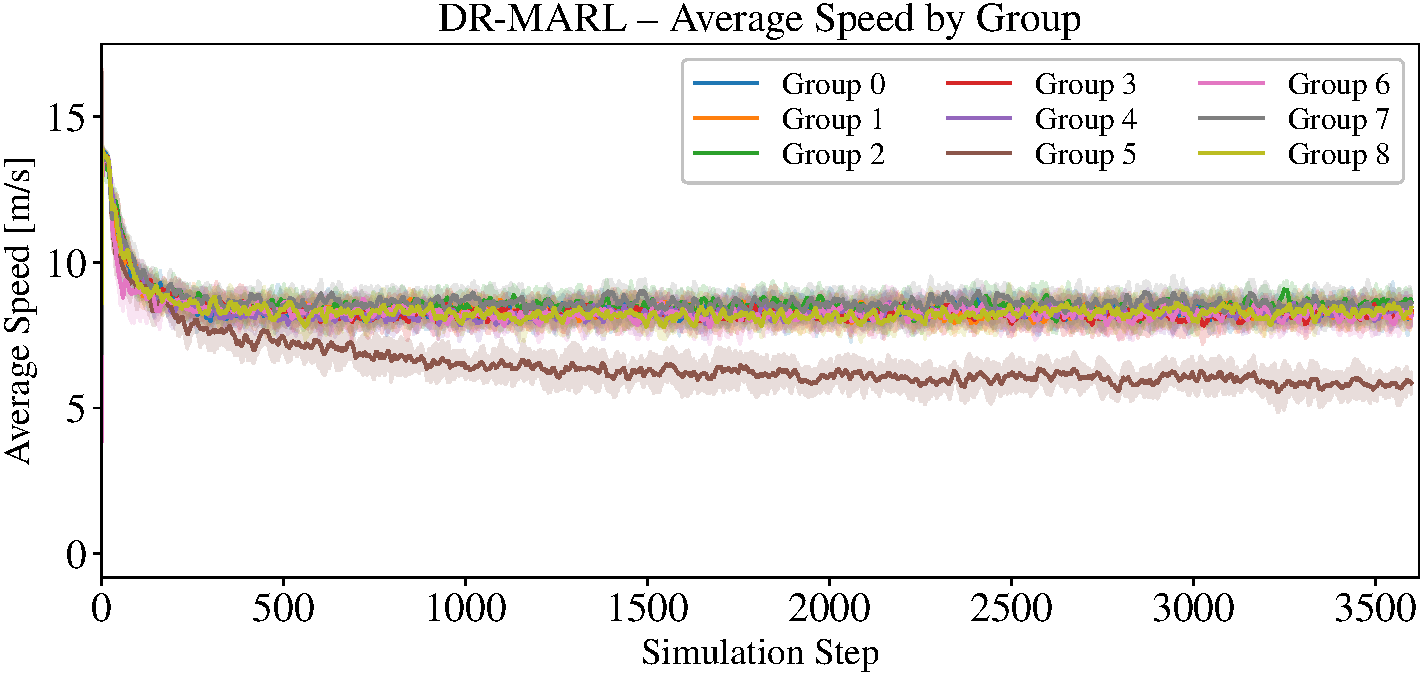
\includegraphics[width=1.0\linewidth]{drmarl_speed_by_group.pdf}
        \caption{Average speed over time under DR-MARL.}
        \label{fig:speed_robust}
    \end{minipage}
\end{figure*}

\begin{figure*}[t!]
    \centering
    \begin{minipage}{0.48\textwidth}
        \centering
        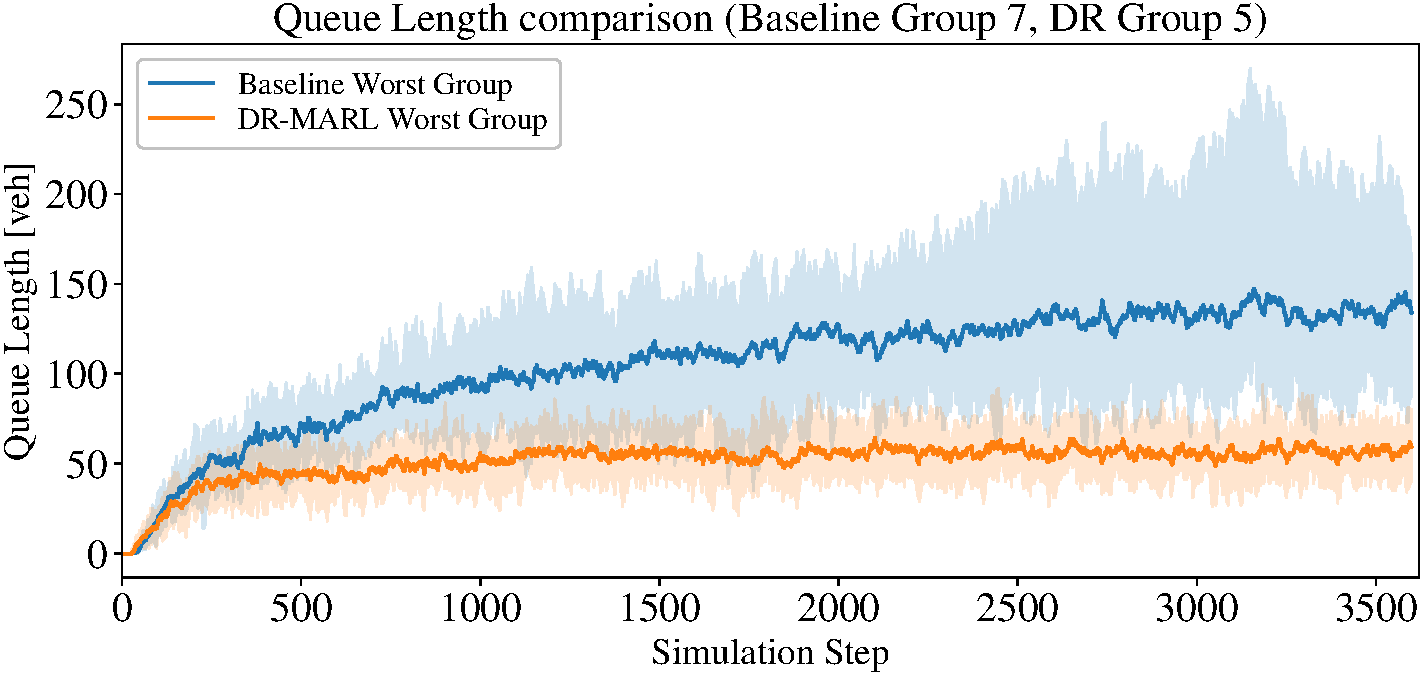
\includegraphics[width=1.0\linewidth]{manual_worst_queue.pdf}
        \caption{Queue length for the worst-performing groups.}
        \label{fig:queue_worst}
    \end{minipage}\hfill
    \begin{minipage}{0.48\textwidth}
        \centering
        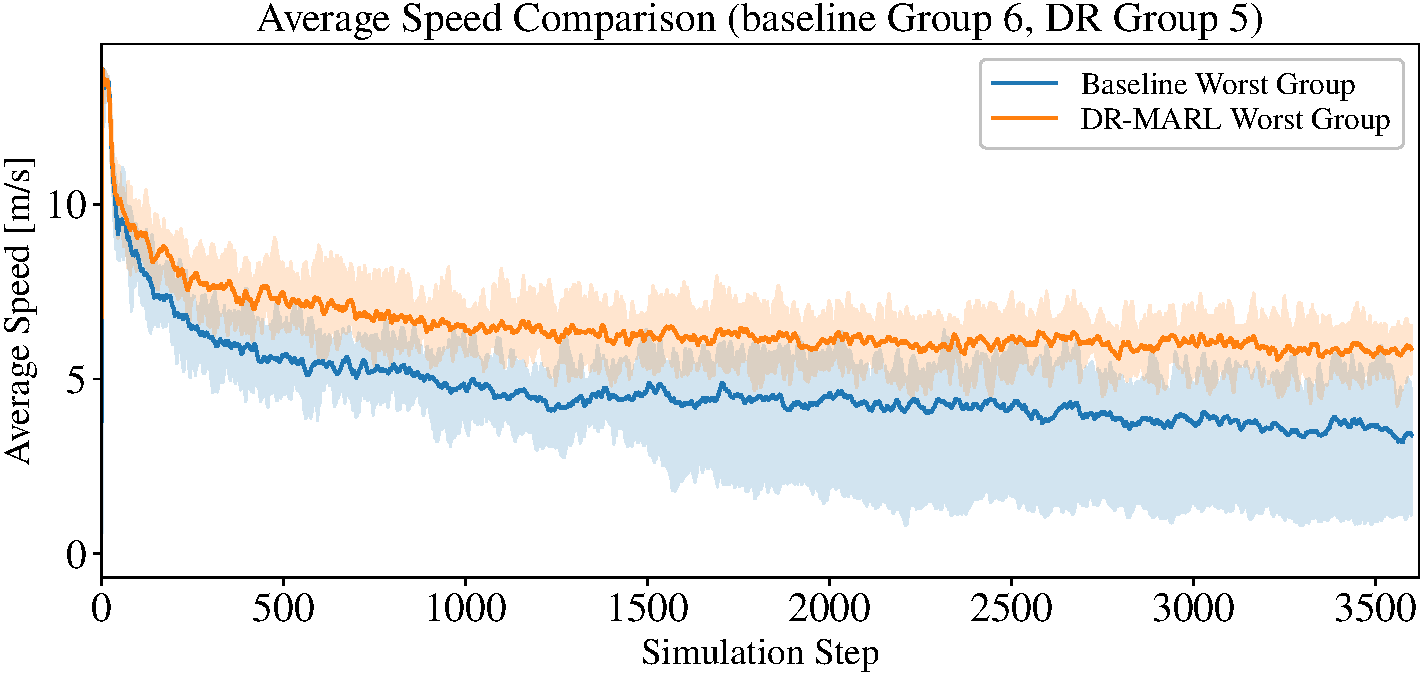
\includegraphics[width=1.0\linewidth]{manual_worst_speed.pdf}
        \caption{Average speed for the worst-performing groups.}
        \label{fig:speed_worst}
    \end{minipage}
\end{figure*}




\subsection{Training protocol}
\label{subsec:training-protocol}

The baseline MARL controller uses an episode horizon of $H = 900$\,s. Each training iteration collects $10$ rollouts, and training runs for $3000$ iterations from scratch. 
For the CB-WCE, episodes span multiple windows  $T_{\mathrm{win}} =$ \SI{600}{\second} to let the estimator observe long-term scenario-selection effects. We use $H_{\text{WCE}} = 9600$\,s, $8$ rollouts per iteration, and $50$ iterations. The $K=8$ scenarios switch per window based on estimator weights. 
The DR-MARL model uses the same multi-window setup ($H_{\text{DR}}= 9600$\,s), with $2$ rollouts per iteration over $400$ iterations, initialized from the trained baseline and updated via the CB-WCE's adaptive scenario selection.

\subsection{Baselines and Evaluation Metrics}
\label{subsec:baseline_eval}
We compare two controllers: the expectation-maximizing \textbf{PPO MARL} baseline (Section~\ref{sec:problem}), and \textbf{DR-MARL}, which uses the same architecture retrained via CB-WCE under the eight demand scenarios. Performance is evaluated using standard network-level metrics: total \textbf{queue length} and \textbf{average speed}. To assess robustness across the demand groups, we compute the horizon-average of each metric per group and report the relative improvement of DR-MARL over the baseline in the following section.




\section{Results and Discussion}



We compare the baseline MARL controller and the DR-MARL controller on the seven synthetic traffic-demand groups, the pNEUMA traffic demand introduction in Section~\ref{subsec:robust-objective}, and on one additional group derived from the enriched Sioux Falls scenario~\citep{chakirov2014enriched}. For the latter, we consider a subnetwork in Sioux Falls that is consistent with our $3\times3 $ grid and normalize the total demand to \SI{5000}{veh/h}. It is used exclusively for evaluation as an independent, previously unseen demand pattern for both controllers. For each controller and each group $k\in\{0,\dots,8\}$, we run $10$ independent evaluation rollouts of length $H_{\mathrm{eval}} = 3600$\,s. During a rollout, the demand is fixed to group $k$ for the full horizon, the learned policy is kept fixed, and only the stochasticity in vehicle generation and microscopic dynamics varies across rollouts. 

Figures~\ref{fig:queue_baseline} and~\ref{fig:queue_robust} show the evolution of network-wide queue length over time for all nine groups under the baseline MARL controller and the DR-MARL controller. Each coloured line corresponds to the per-timestep mean queue length (over 10 rollouts) for a single demand group. Under the baseline MARL controller, queues diverge substantially across groups and reach the highest levels for group~7. Under DR-MARL, the curves are consistently shifted downward: all groups stabilize at noticeably lower queue levels, with group~5 being the heaviest but still far below the baseline MARL controllers worst case. The unseen Sioux Falls group (group~8) exhibits a similar clear reduction in queues under DR-MARL.


Figures~\ref{fig:speed_baseline} and~\ref{fig:speed_robust} report the corresponding average speeds. Under the baseline MARL controller, steady-state speeds vary between roughly \SIrange{4.5}{7}{m/s} depending on the group, with groups~6 and~7 performing worst. Under DR-MARL, all nine groups attain higher steady-state speeds, typically around \SI{8}{m/s} or above, with only group~5 clearly below this level. The Sioux Falls group again follows this pattern, confirming that the DR-MARL policy generalises better than the baseline to an unseen demand distribution.




Table~\ref{tab:comp} summarizes these results numerically, reporting the horizon- and rollout-averaged metrics alongside their relative changes. DR-MARL substantially reduces queue lengths (by roughly $21$–$69$\%) and increases average speeds (by $16$–$77$\%) across all groups. Notably, the largest queue reduction ($-68.7$\%) occurs in group~7, while the highest speed gains ($+76.7$\%) are seen in groups~6 and~7. For the unseen Sioux Falls pattern (group~8), DR-MARL also reduces queues by $41.6$\% and increases speed by $22.9$\%, confirming strong generalization.

\begin{table}[t!]
    \centering
    \caption{Comparison of MARL and DR-MARL performance (horizon-and-rollout-averaged).}
    \label{tab:comp}
    \resizebox{1.0\linewidth}{!}{
    \begin{tabular}{|c|ccc|ccc|}
        \hline
        & \multicolumn{3}{c|}{Queue length} & \multicolumn{3}{c|}{Average speed} \\
        \cline{2-7}
        Group & MARL & DR-MARL & Change & MARL & DR-MARL & Change \\
        \hline
        0 & 72.287 & 40.137 & -44.5\% & 6.882 & 8.411 & +22.2\% \\
        1 & 70.318 & 39.959 & -43.2\% & 6.925 & 8.404 & +21.3\% \\
        2 & 76.829 & 35.250 & -54.1\% & 6.297 & 8.571 & +36.1\% \\
        3 & 76.062 & 38.528 & -49.3\% & 5.429 & 8.358 & +54.0\% \\
        4 & 67.008 & 40.250 & -39.9\% & 6.105 & 8.347 & +36.7\% \\
        5 & 64.620 & 51.302 & -20.6\% & 5.647 & 6.524 & +15.5\% \\
        6 & 60.094 & 39.914 & -33.6\% & 4.714 & 8.330 & +76.7\% \\
        7 & 105.153 & 32.932 & -68.7\% & 4.910 & 8.685 & +76.7\% \\ 
        8 & 65.711 & 38.372 & -41.6\% & 6.795 & 8.353 & +22.9\% \\
        \hline
    \end{tabular}
    }
\end{table}


As discussed in Section~\ref{subsec:robust-objective}, our main interest lies in improving the worst-case performance $J_{\mathrm{worst}}$ across demand groups. From Table~\ref{tab:comp}, we identify group~7 as the worst-performing group in terms of average queue length and group~6 as the worst for average speed under the baseline MARL controller, whereas group~5 is the worst group for both metrics under the DR-MARL controller. Comparing these worst cases, the DR-MARL controller reduces the worst observed average queue length by about $51.2\,\%$ (baseline group~7 vs.\ DR-MARL group~5) and increases the worst observed average speed by about $38.4\,\%$ (baseline group~6 vs.\ DR-MARL group~5). Figures~\ref{fig:queue_worst} and~\ref{fig:speed_worst} visualize the evolution of queues and speeds over time for these worst-case baseline and DR-MARL groups. The DR-MARL trajectories maintain substantially lower queues and higher speeds over most of the horizon, indicating that the contextual-bandit reweighting improves the policy precisely on its most challenging scenarios.





Retraining with CB-WCE improves typical and worst-case performance without altering the MARL architecture or reward. DR-MARL achieves large gains on the hardest baseline groups and generalizes to the unseen Sioux Falls pattern. Although slight overlaps in Figures~\ref{fig:queue_worst} and~\ref{fig:speed_worst} indicate some DR-MARL rollouts perform similarly to the baseline due to simulation stochasticity, the overall performance distribution shifts markedly in a favorable direction.

\section{Conclusion and Outlook}
\label{sec:conclusion}

We proposed a DR-MARL framework for traffic-signal control, evaluated on a calibrated $3\times3$ grid. By introducing a CB-WCE to select adversarial demand mixtures during fine-tuning, we enhanced the robustness of a baseline MARL controller. Across nine scenarios, DR-MARL improved average speeds by $16$–$77,\%$ and reduced queues by $21$–$69,\%$, yielding significant gains in both typical ($J_{\mathrm{avg}}$) and worst-case ($J_{\mathrm{worst}}$) performance.

Limitations include the reliance on a finite set of scenarios over a stylized grid and freezing the estimator during fine-tuning, which anchors it to the baseline's worst cases. Future work will extend this framework to larger, heterogeneous networks and allow the worst-case estimator to continuously adapt alongside the DR-MARL policy.
\footnotesize
\balance 
\bibliography{ifacconf}

\end{document}
